\documentclass{standalone}
\usepackage{tikz}
\usetikzlibrary{patterns, positioning}
\usepackage[sfdefault]{ClearSans} %% option 'sfdefault' activates Clear Sans as the default text font
\usepackage[T1]{fontenc}

\begin{document}
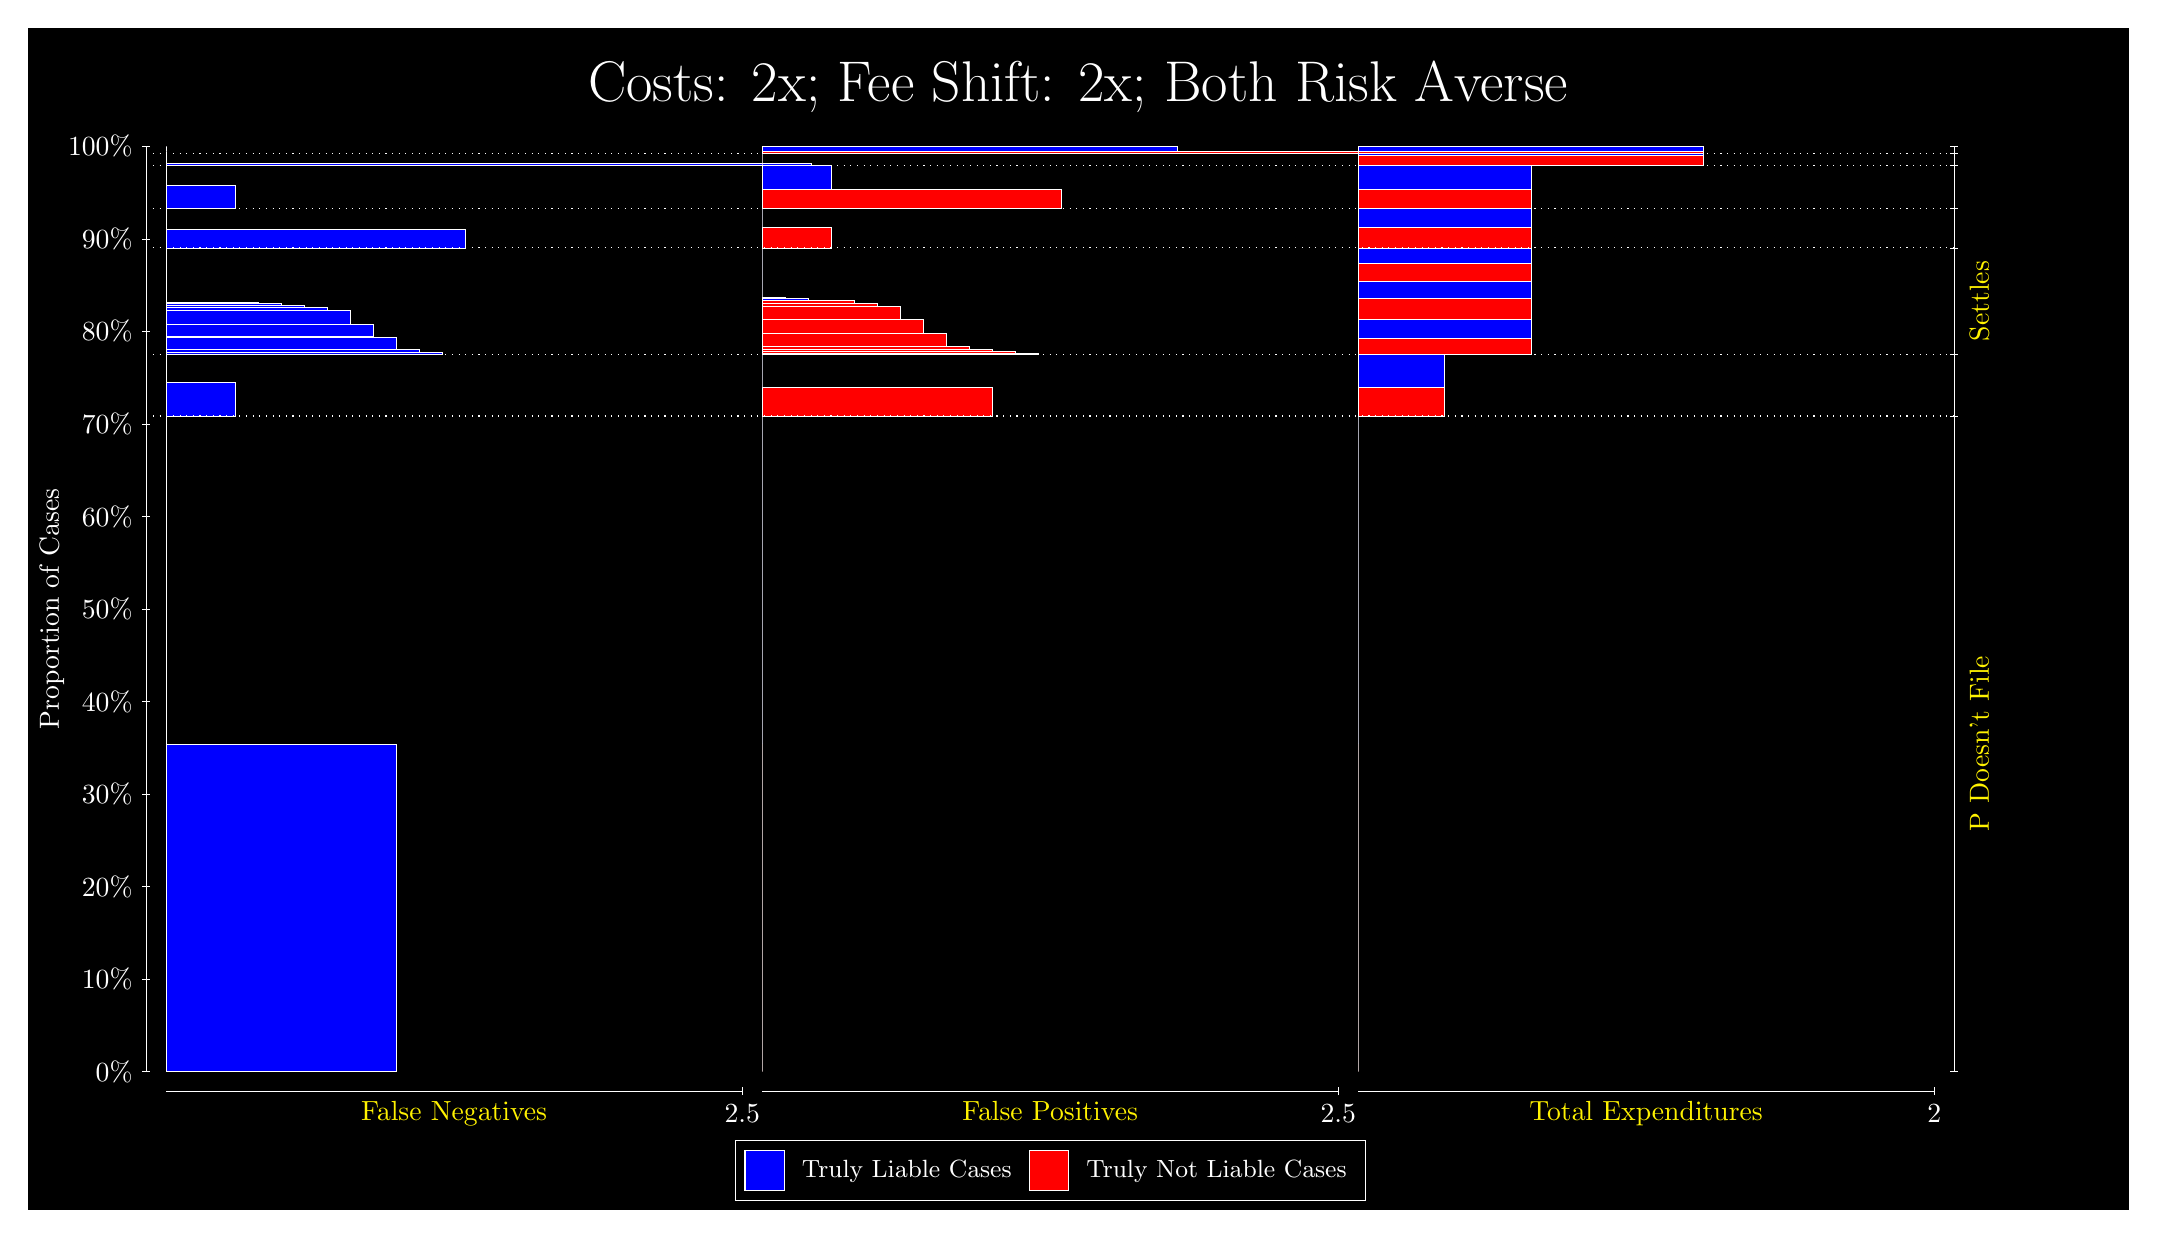
\begin{tikzpicture}
\draw[fill=black] (0,0) rectangle (26.667,15);
\draw[text=white] (0,13.5) rectangle (26.667,15) node[midway] {\huge Costs: 2x; Fee Shift: 2x; Both Risk Averse};
\draw[white, very thin] (1.5,1.75) -- (1.5,13.5);
\node[rotate=90, text=white, anchor=center] at (0.3, 7.625) {Proportion of Cases};
\draw[white, very thin] (1.45,1.75) -- (1.55,1.75);
\node[text=white, anchor=east] at (1.45, 1.75) {0\%};
\draw[white, very thin] (1.45,2.925) -- (1.55,2.925);
\node[text=white, anchor=east] at (1.45, 2.925) {10\%};
\draw[white, very thin] (1.45,4.1) -- (1.55,4.1);
\node[text=white, anchor=east] at (1.45, 4.1) {20\%};
\draw[white, very thin] (1.45,5.275) -- (1.55,5.275);
\node[text=white, anchor=east] at (1.45, 5.275) {30\%};
\draw[white, very thin] (1.45,6.45) -- (1.55,6.45);
\node[text=white, anchor=east] at (1.45, 6.45) {40\%};
\draw[white, very thin] (1.45,7.625) -- (1.55,7.625);
\node[text=white, anchor=east] at (1.45, 7.625) {50\%};
\draw[white, very thin] (1.45,8.8) -- (1.55,8.8);
\node[text=white, anchor=east] at (1.45, 8.8) {60\%};
\draw[white, very thin] (1.45,9.975) -- (1.55,9.975);
\node[text=white, anchor=east] at (1.45, 9.975) {70\%};
\draw[white, very thin] (1.45,11.15) -- (1.55,11.15);
\node[text=white, anchor=east] at (1.45, 11.15) {80\%};
\draw[white, very thin] (1.45,12.325) -- (1.55,12.325);
\node[text=white, anchor=east] at (1.45, 12.325) {90\%};
\draw[white, very thin] (1.45,13.5) -- (1.55,13.5);
\node[text=white, anchor=east] at (1.45, 13.5) {100\%};

\draw[white, very thin] (24.457,1.75) -- (24.457,13.5);
\draw[white, very thin] (24.407,1.75) -- (24.507,1.75);
\node[anchor=west] at (24.407, 1.75) {};
\draw[white, very thin] (24.407,10.075) -- (24.507,10.075);
\node[anchor=west] at (24.407, 10.075) {};
\draw[white, very thin] (24.407,10.861) -- (24.507,10.861);
\node[anchor=west] at (24.407, 10.861) {};
\draw[white, very thin] (24.407,12.211) -- (24.507,12.211);
\node[anchor=west] at (24.407, 12.211) {};
\draw[white, very thin] (24.407,12.707) -- (24.507,12.707);
\node[anchor=west] at (24.407, 12.707) {};
\draw[white, very thin] (24.407,13.261) -- (24.507,13.261);
\node[anchor=west] at (24.407, 13.261) {};
\draw[white, very thin] (24.407,13.41) -- (24.507,13.41);
\node[anchor=west] at (24.407, 13.41) {};
\draw[white, very thin] (24.407,13.5) -- (24.507,13.5);
\node[anchor=west] at (24.407, 13.5) {};

\draw[white, very thin, fill=blue] (1.75,1.75) rectangle (4.6775,5.9123);
\draw[white, very thin, fill=red] (1.75,5.9123) rectangle (1.75,10.075);
\draw[white, very thin, fill=blue] (1.75,10.075) rectangle (2.6283,10.501);
\draw[white, very thin, fill=red] (1.75,10.501) rectangle (1.75,10.861);
\draw[white, very thin, fill=blue] (1.75,10.861) rectangle (5.2631,10.89);
\draw[white, very thin, fill=blue] (1.75,10.89) rectangle (4.9703,10.917);
\draw[white, very thin, fill=blue] (1.75,10.917) rectangle (4.6775,11.074);
\draw[white, very thin, fill=blue] (1.75,11.074) rectangle (4.3848,11.087);
\draw[white, very thin, fill=blue] (1.75,11.087) rectangle (4.3848,11.24);
\draw[white, very thin, fill=blue] (1.75,11.24) rectangle (4.092,11.421);
\draw[white, very thin, fill=blue] (1.75,11.421) rectangle (3.7993,11.452);
\draw[white, very thin, fill=blue] (1.75,11.452) rectangle (3.5065,11.487);
\draw[white, very thin, fill=blue] (1.75,11.487) rectangle (3.2138,11.507);
\draw[white, very thin, fill=blue] (1.75,11.507) rectangle (2.921,11.523);
\draw[white, very thin, fill=red] (1.75,11.523) rectangle (1.75,12.211);
\draw[white, very thin, fill=blue] (1.75,12.211) rectangle (5.5558,12.444);
\draw[white, very thin, fill=red] (1.75,12.444) rectangle (1.75,12.707);
\draw[white, very thin, fill=blue] (1.75,12.707) rectangle (2.6283,13.009);
\draw[white, very thin, fill=red] (1.75,13.009) rectangle (1.75,13.261);
\draw[white, very thin, fill=blue] (1.75,13.261) rectangle (9.9471,13.283);
\draw[white, very thin, fill=red] (1.75,13.283) rectangle (1.75,13.41);
\draw[white, very thin, fill=red] (1.75,13.41) rectangle (1.75,13.432);
\draw[white, very thin, fill=blue] (1.75,13.432) rectangle (1.75,13.5);
\draw[white, very thin, fill=red] (9.3189,1.75) rectangle (9.3189,5.9124);
\draw[white, very thin, fill=blue] (9.3189,5.9124) rectangle (9.3189,10.075);
\draw[white, very thin, fill=red] (9.3189,10.075) rectangle (12.246,10.435);
\draw[white, very thin, fill=blue] (9.3189,10.435) rectangle (9.3189,10.861);
\draw[white, very thin, fill=red] (9.3189,10.861) rectangle (12.832,10.877);
\draw[white, very thin, fill=red] (9.3189,10.877) rectangle (12.539,10.894);
\draw[white, very thin, fill=red] (9.3189,10.894) rectangle (12.246,10.927);
\draw[white, very thin, fill=red] (9.3189,10.927) rectangle (11.954,10.963);
\draw[white, very thin, fill=red] (9.3189,10.963) rectangle (11.661,11.121);
\draw[white, very thin, fill=red] (9.3189,11.121) rectangle (11.368,11.3);
\draw[white, very thin, fill=red] (9.3189,11.3) rectangle (11.075,11.469);
\draw[white, very thin, fill=red] (9.3189,11.469) rectangle (10.783,11.507);
\draw[white, very thin, fill=red] (9.3189,11.507) rectangle (10.49,11.549);
\draw[white, very thin, fill=blue] (9.3189,11.549) rectangle (9.9044,11.564);
\draw[white, very thin, fill=blue] (9.3189,11.564) rectangle (9.6116,11.584);
\draw[white, very thin, fill=blue] (9.3189,11.584) rectangle (9.3189,12.211);
\draw[white, very thin, fill=red] (9.3189,12.211) rectangle (10.197,12.474);
\draw[white, very thin, fill=blue] (9.3189,12.474) rectangle (9.3189,12.707);
\draw[white, very thin, fill=red] (9.3189,12.707) rectangle (13.125,12.96);
\draw[white, very thin, fill=blue] (9.3189,12.96) rectangle (10.197,13.261);
\draw[white, very thin, fill=red] (9.3189,13.261) rectangle (9.3189,13.389);
\draw[white, very thin, fill=blue] (9.3189,13.389) rectangle (9.3189,13.41);
\draw[white, very thin, fill=red] (9.3189,13.41) rectangle (17.516,13.432);
\draw[white, very thin, fill=blue] (9.3189,13.432) rectangle (14.588,13.5);
\draw[white, very thin, fill=red] (16.888,1.75) rectangle (16.888,5.9124);
\draw[white, very thin, fill=blue] (16.888,5.9124) rectangle (16.888,10.075);
\draw[white, very thin, fill=red] (16.888,10.075) rectangle (17.986,10.435);
\draw[white, very thin, fill=blue] (16.888,10.435) rectangle (17.986,10.861);
\draw[white, very thin, fill=red] (16.888,10.861) rectangle (19.083,11.068);
\draw[white, very thin, fill=blue] (16.888,11.068) rectangle (19.083,11.304);
\draw[white, very thin, fill=red] (16.888,11.304) rectangle (19.083,11.566);
\draw[white, very thin, fill=blue] (16.888,11.566) rectangle (19.083,11.792);
\draw[white, very thin, fill=red] (16.888,11.792) rectangle (19.083,12.011);
\draw[white, very thin, fill=blue] (16.888,12.011) rectangle (19.083,12.211);
\draw[white, very thin, fill=red] (16.888,12.211) rectangle (19.083,12.474);
\draw[white, very thin, fill=blue] (16.888,12.474) rectangle (19.083,12.707);
\draw[white, very thin, fill=red] (16.888,12.707) rectangle (19.083,12.96);
\draw[white, very thin, fill=blue] (16.888,12.96) rectangle (19.083,13.261);
\draw[white, very thin, fill=red] (16.888,13.261) rectangle (21.279,13.389);
\draw[white, very thin, fill=blue] (16.888,13.389) rectangle (21.279,13.41);
\draw[white, very thin, fill=red] (16.888,13.41) rectangle (21.279,13.432);
\draw[white, very thin, fill=blue] (16.888,13.432) rectangle (21.279,13.5);
\draw[white, dotted] (1.5,10.075) -- (24.457,10.075);
\draw[white, dotted] (1.5,10.861) -- (24.457,10.861);
\draw[white, dotted] (1.5,12.211) -- (24.457,12.211);
\draw[white, dotted] (1.5,12.707) -- (24.457,12.707);
\draw[white, dotted] (1.5,13.261) -- (24.457,13.261);
\draw[white, dotted] (1.5,13.41) -- (24.457,13.41);
\draw[white, very thin] (1.75,1.5) -- (9.0689,1.5);
\node[text=yellow, anchor=north] at (5.4094, 1.5) {False Negatives};
\draw[white, very thin] (9.0689,1.45) -- (9.0689,1.55);
\node[text=white, anchor=north] at (9.0689, 1.45) {2.5};

\draw[white, very thin] (9.3189,1.5) -- (16.638,1.5);
\node[text=yellow, anchor=north] at (12.978, 1.5) {False Positives};
\draw[white, very thin] (16.638,1.45) -- (16.638,1.55);
\node[text=white, anchor=north] at (16.638, 1.45) {2.5};

\draw[white, very thin] (16.888,1.5) -- (24.207,1.5);
\node[text=yellow, anchor=north] at (20.547, 1.5) {Total Expenditures};
\draw[white, very thin] (24.207,1.45) -- (24.207,1.55);
\node[text=white, anchor=north] at (24.207, 1.45) {2};

\node[text=yellow, centered, rotate=90] at (24.777, 5.9123) {P Doesn't File};

\node[text=yellow, centered, rotate=90] at (24.777, 11.536) {Settles};





\draw (12.978300999999998,1.5) node[draw=none] (baseCoordinate) {};
\begin{scope}[align=center]
        \matrix[scale=0.5, draw=white, below=0.5cm of baseCoordinate, nodes={draw}, column sep=0.1cm]{
            \node[rectangle, draw, minimum width=0.5cm, minimum height=0.5cm, fill=blue] {}; &
            \node[draw=none, font=\small, text=white] (B) {Truly Liable Cases}; &
            \node[rectangle, draw, minimum width=0.5cm, minimum height=0.5cm, fill=red] {}; &
            \node[draw=none, font=\small, text=white] (B) {Truly Not Liable Cases}; \\
            };
\end{scope}

\end{tikzpicture}
\end{document}